\documentclass{standalone}
\usepackage{tikz}
\usetikzlibrary{patterns, positioning}
\usepackage[sfdefault]{ClearSans} %% option 'sfdefault' activates Clear Sans as the default text font
\usepackage[T1]{fontenc}

\begin{document}
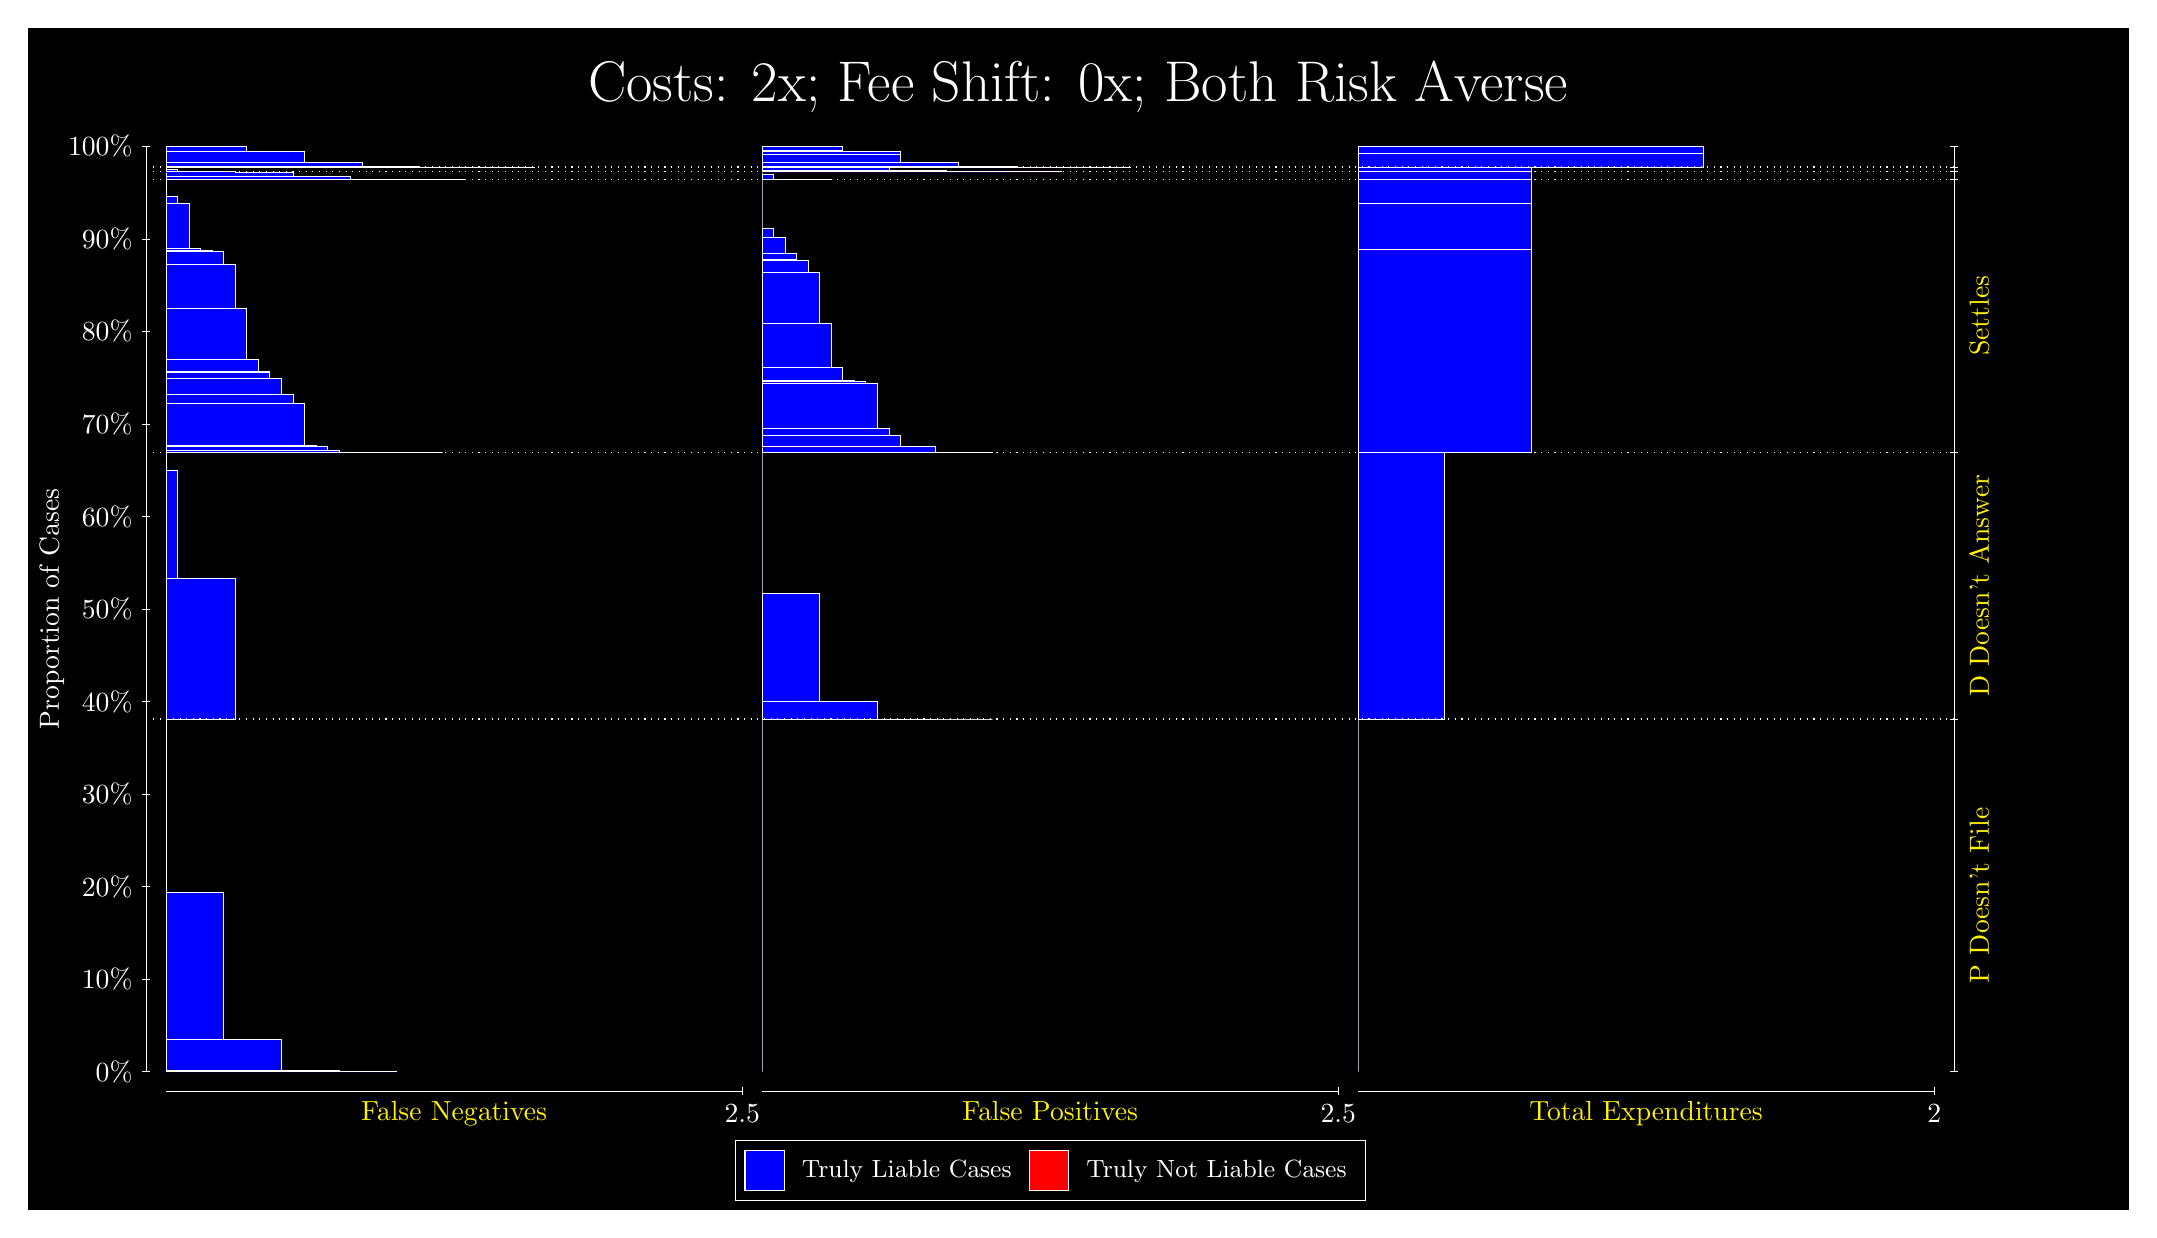
\begin{tikzpicture}
\draw[fill=black] (0,0) rectangle (26.667,15);
\draw[text=white] (0,13.5) rectangle (26.667,15) node[midway] {\huge Costs: 2x; Fee Shift: 0x; Both Risk Averse};
\draw[white, very thin] (1.5,1.75) -- (1.5,13.5);
\node[rotate=90, text=white, anchor=center] at (0.3, 7.625) {Proportion of Cases};
\draw[white, very thin] (1.45,1.75) -- (1.55,1.75);
\node[text=white, anchor=east] at (1.45, 1.75) {0\%};
\draw[white, very thin] (1.45,2.925) -- (1.55,2.925);
\node[text=white, anchor=east] at (1.45, 2.925) {10\%};
\draw[white, very thin] (1.45,4.1) -- (1.55,4.1);
\node[text=white, anchor=east] at (1.45, 4.1) {20\%};
\draw[white, very thin] (1.45,5.275) -- (1.55,5.275);
\node[text=white, anchor=east] at (1.45, 5.275) {30\%};
\draw[white, very thin] (1.45,6.45) -- (1.55,6.45);
\node[text=white, anchor=east] at (1.45, 6.45) {40\%};
\draw[white, very thin] (1.45,7.625) -- (1.55,7.625);
\node[text=white, anchor=east] at (1.45, 7.625) {50\%};
\draw[white, very thin] (1.45,8.8) -- (1.55,8.8);
\node[text=white, anchor=east] at (1.45, 8.8) {60\%};
\draw[white, very thin] (1.45,9.975) -- (1.55,9.975);
\node[text=white, anchor=east] at (1.45, 9.975) {70\%};
\draw[white, very thin] (1.45,11.15) -- (1.55,11.15);
\node[text=white, anchor=east] at (1.45, 11.15) {80\%};
\draw[white, very thin] (1.45,12.325) -- (1.55,12.325);
\node[text=white, anchor=east] at (1.45, 12.325) {90\%};
\draw[white, very thin] (1.45,13.5) -- (1.55,13.5);
\node[text=white, anchor=east] at (1.45, 13.5) {100\%};

\draw[white, very thin] (24.457,1.75) -- (24.457,13.5);
\draw[white, very thin] (24.407,1.75) -- (24.507,1.75);
\node[anchor=west] at (24.407, 1.75) {};
\draw[white, very thin] (24.407,6.2271) -- (24.507,6.2271);
\node[anchor=west] at (24.407, 6.2271) {};
\draw[white, very thin] (24.407,9.6138) -- (24.507,9.6138);
\node[anchor=west] at (24.407, 9.6138) {};
\draw[white, very thin] (24.407,13.082) -- (24.507,13.082);
\node[anchor=west] at (24.407, 13.082) {};
\draw[white, very thin] (24.407,13.177) -- (24.507,13.177);
\node[anchor=west] at (24.407, 13.177) {};
\draw[white, very thin] (24.407,13.237) -- (24.507,13.237);
\node[anchor=west] at (24.407, 13.237) {};
\draw[white, very thin] (24.407,13.5) -- (24.507,13.5);
\node[anchor=west] at (24.407, 13.5) {};

\draw[white, very thin, fill=blue] (1.75,1.75) rectangle (4.6775,1.7501);
\draw[white, very thin, fill=blue] (1.75,1.7501) rectangle (3.9457,1.7644);
\draw[white, very thin, fill=blue] (1.75,1.7644) rectangle (3.2138,2.163);
\draw[white, very thin, fill=blue] (1.75,2.163) rectangle (2.4819,4.0274);
\draw[white, very thin, fill=red] (1.75,4.0274) rectangle (1.75,4.0274);
\draw[white, very thin, fill=blue] (1.75,4.0274) rectangle (1.75,6.2271);
\draw[white, very thin, fill=blue] (1.75,6.2271) rectangle (2.6283,8.0192);
\draw[white, very thin, fill=blue] (1.75,8.0192) rectangle (1.8964,9.3896);
\draw[white, very thin, fill=red] (1.75,9.3896) rectangle (1.75,9.3896);
\draw[white, very thin, fill=blue] (1.75,9.3896) rectangle (1.75,9.6138);
\draw[white, very thin, fill=blue] (1.75,9.6138) rectangle (5.2631,9.6138);
\draw[white, very thin, fill=blue] (1.75,9.6138) rectangle (4.6775,9.6139);
\draw[white, very thin, fill=blue] (1.75,9.6139) rectangle (4.5312,9.6152);
\draw[white, very thin, fill=blue] (1.75,9.6152) rectangle (4.3848,9.6152);
\draw[white, very thin, fill=blue] (1.75,9.6152) rectangle (4.092,9.6154);
\draw[white, very thin, fill=blue] (1.75,9.6154) rectangle (3.9457,9.6437);
\draw[white, very thin, fill=blue] (1.75,9.6437) rectangle (3.7993,9.6948);
\draw[white, very thin, fill=blue] (1.75,9.6948) rectangle (3.6529,9.7021);
\draw[white, very thin, fill=blue] (1.75,9.7021) rectangle (3.5065,10.239);
\draw[white, very thin, fill=blue] (1.75,10.239) rectangle (3.3602,10.345);
\draw[white, very thin, fill=blue] (1.75,10.345) rectangle (3.2138,10.556);
\draw[white, very thin, fill=blue] (1.75,10.556) rectangle (3.0674,10.631);
\draw[white, very thin, fill=blue] (1.75,10.631) rectangle (3.0674,10.642);
\draw[white, very thin, fill=blue] (1.75,10.642) rectangle (2.921,10.795);
\draw[white, very thin, fill=blue] (1.75,10.795) rectangle (2.7746,11.437);
\draw[white, very thin, fill=blue] (1.75,11.437) rectangle (2.6283,12.002);
\draw[white, very thin, fill=blue] (1.75,12.002) rectangle (2.4819,12.165);
\draw[white, very thin, fill=blue] (1.75,12.165) rectangle (2.3355,12.183);
\draw[white, very thin, fill=blue] (1.75,12.183) rectangle (2.3355,12.183);
\draw[white, very thin, fill=blue] (1.75,12.183) rectangle (2.1891,12.21);
\draw[white, very thin, fill=blue] (1.75,12.21) rectangle (2.0428,12.779);
\draw[white, very thin, fill=blue] (1.75,12.779) rectangle (1.8964,12.864);
\draw[white, very thin, fill=red] (1.75,12.864) rectangle (1.75,12.864);
\draw[white, very thin, fill=blue] (1.75,12.864) rectangle (1.75,13.082);
\draw[white, very thin, fill=blue] (1.75,13.082) rectangle (5.5558,13.082);
\draw[white, very thin, fill=blue] (1.75,13.082) rectangle (4.8239,13.082);
\draw[white, very thin, fill=blue] (1.75,13.082) rectangle (4.092,13.117);
\draw[white, very thin, fill=blue] (1.75,13.117) rectangle (3.3602,13.175);
\draw[white, very thin, fill=blue] (1.75,13.175) rectangle (2.6283,13.177);
\draw[white, very thin, fill=red] (1.75,13.177) rectangle (1.75,13.177);
\draw[white, very thin, fill=blue] (1.75,13.177) rectangle (2.6283,13.178);
\draw[white, very thin, fill=blue] (1.75,13.178) rectangle (1.8964,13.214);
\draw[white, very thin, fill=red] (1.75,13.214) rectangle (1.75,13.214);
\draw[white, very thin, fill=blue] (1.75,13.214) rectangle (1.75,13.237);
\draw[white, very thin, fill=blue] (1.75,13.237) rectangle (6.4341,13.237);
\draw[white, very thin, fill=blue] (1.75,13.237) rectangle (5.7022,13.237);
\draw[white, very thin, fill=blue] (1.75,13.237) rectangle (4.9703,13.241);
\draw[white, very thin, fill=blue] (1.75,13.241) rectangle (4.2384,13.302);
\draw[white, very thin, fill=blue] (1.75,13.302) rectangle (3.5065,13.435);
\draw[white, very thin, fill=blue] (1.75,13.435) rectangle (2.7746,13.496);
\draw[white, very thin, fill=blue] (1.75,13.496) rectangle (2.0428,13.5);
\draw[white, very thin, fill=red] (1.75,13.5) rectangle (1.75,13.5);
\draw[white, very thin, fill=blue] (1.75,13.5) rectangle (1.75,13.5);
\draw[white, very thin, fill=red] (9.3189,1.75) rectangle (9.3189,1.75);
\draw[white, very thin, fill=blue] (9.3189,1.75) rectangle (9.3189,6.2271);
\draw[white, very thin, fill=red] (9.3189,6.2271) rectangle (12.246,6.2271);
\draw[white, very thin, fill=blue] (9.3189,6.2271) rectangle (12.246,6.2271);
\draw[white, very thin, fill=blue] (9.3189,6.2271) rectangle (11.515,6.2282);
\draw[white, very thin, fill=blue] (9.3189,6.2282) rectangle (10.783,6.4513);
\draw[white, very thin, fill=blue] (9.3189,6.4513) rectangle (10.051,7.8217);
\draw[white, very thin, fill=blue] (9.3189,7.8217) rectangle (9.3189,9.6138);
\draw[white, very thin, fill=red] (9.3189,9.6138) rectangle (12.246,9.6138);
\draw[white, very thin, fill=blue] (9.3189,9.6138) rectangle (12.246,9.6139);
\draw[white, very thin, fill=red] (9.3189,9.6139) rectangle (11.954,9.6139);
\draw[white, very thin, fill=blue] (9.3189,9.6139) rectangle (11.954,9.6139);
\draw[white, very thin, fill=red] (9.3189,9.6139) rectangle (11.661,9.6139);
\draw[white, very thin, fill=blue] (9.3189,9.6139) rectangle (11.661,9.6141);
\draw[white, very thin, fill=blue] (9.3189,9.6141) rectangle (11.515,9.6851);
\draw[white, very thin, fill=red] (9.3189,9.6851) rectangle (11.368,9.6851);
\draw[white, very thin, fill=blue] (9.3189,9.6851) rectangle (11.368,9.6853);
\draw[white, very thin, fill=blue] (9.3189,9.6853) rectangle (11.222,9.6854);
\draw[white, very thin, fill=red] (9.3189,9.6854) rectangle (11.075,9.6854);
\draw[white, very thin, fill=blue] (9.3189,9.6854) rectangle (11.075,9.8321);
\draw[white, very thin, fill=blue] (9.3189,9.8321) rectangle (10.929,9.9169);
\draw[white, very thin, fill=blue] (9.3189,9.9169) rectangle (10.783,10.486);
\draw[white, very thin, fill=blue] (9.3189,10.486) rectangle (10.636,10.513);
\draw[white, very thin, fill=red] (9.3189,10.513) rectangle (10.49,10.513);
\draw[white, very thin, fill=blue] (9.3189,10.513) rectangle (10.49,10.513);
\draw[white, very thin, fill=blue] (9.3189,10.513) rectangle (10.49,10.531);
\draw[white, very thin, fill=blue] (9.3189,10.531) rectangle (10.344,10.693);
\draw[white, very thin, fill=blue] (9.3189,10.693) rectangle (10.197,11.259);
\draw[white, very thin, fill=blue] (9.3189,11.259) rectangle (10.051,11.9);
\draw[white, very thin, fill=blue] (9.3189,11.9) rectangle (9.9044,12.053);
\draw[white, very thin, fill=blue] (9.3189,12.053) rectangle (9.758,12.064);
\draw[white, very thin, fill=blue] (9.3189,12.064) rectangle (9.758,12.139);
\draw[white, very thin, fill=blue] (9.3189,12.139) rectangle (9.6116,12.351);
\draw[white, very thin, fill=blue] (9.3189,12.351) rectangle (9.4652,12.457);
\draw[white, very thin, fill=blue] (9.3189,12.457) rectangle (9.3189,13.082);
\draw[white, very thin, fill=red] (9.3189,13.082) rectangle (10.197,13.082);
\draw[white, very thin, fill=blue] (9.3189,13.082) rectangle (10.197,13.083);
\draw[white, very thin, fill=blue] (9.3189,13.083) rectangle (9.4652,13.141);
\draw[white, very thin, fill=blue] (9.3189,13.141) rectangle (9.3189,13.177);
\draw[white, very thin, fill=red] (9.3189,13.177) rectangle (13.125,13.177);
\draw[white, very thin, fill=blue] (9.3189,13.177) rectangle (13.125,13.177);
\draw[white, very thin, fill=blue] (9.3189,13.177) rectangle (12.393,13.177);
\draw[white, very thin, fill=blue] (9.3189,13.177) rectangle (11.661,13.199);
\draw[white, very thin, fill=blue] (9.3189,13.199) rectangle (10.929,13.236);
\draw[white, very thin, fill=blue] (9.3189,13.236) rectangle (10.197,13.237);
\draw[white, very thin, fill=red] (9.3189,13.237) rectangle (14.003,13.237);
\draw[white, very thin, fill=blue] (9.3189,13.237) rectangle (14.003,13.237);
\draw[white, very thin, fill=red] (9.3189,13.237) rectangle (13.271,13.237);
\draw[white, very thin, fill=blue] (9.3189,13.237) rectangle (13.271,13.237);
\draw[white, very thin, fill=red] (9.3189,13.237) rectangle (12.539,13.237);
\draw[white, very thin, fill=blue] (9.3189,13.237) rectangle (12.539,13.241);
\draw[white, very thin, fill=blue] (9.3189,13.241) rectangle (11.807,13.302);
\draw[white, very thin, fill=red] (9.3189,13.302) rectangle (11.807,13.302);
\draw[white, very thin, fill=blue] (9.3189,13.302) rectangle (11.807,13.302);
\draw[white, very thin, fill=blue] (9.3189,13.302) rectangle (11.075,13.398);
\draw[white, very thin, fill=red] (9.3189,13.398) rectangle (11.075,13.398);
\draw[white, very thin, fill=blue] (9.3189,13.398) rectangle (11.075,13.435);
\draw[white, very thin, fill=blue] (9.3189,13.435) rectangle (10.344,13.451);
\draw[white, very thin, fill=blue] (9.3189,13.451) rectangle (10.344,13.496);
\draw[white, very thin, fill=blue] (9.3189,13.496) rectangle (9.6116,13.496);
\draw[white, very thin, fill=blue] (9.3189,13.496) rectangle (9.6116,13.5);
\draw[white, very thin, fill=blue] (9.3189,13.5) rectangle (9.3189,13.5);
\draw[white, very thin, fill=red] (16.888,1.75) rectangle (16.888,1.75);
\draw[white, very thin, fill=blue] (16.888,1.75) rectangle (16.888,6.2271);
\draw[white, very thin, fill=red] (16.888,6.2271) rectangle (17.986,6.2271);
\draw[white, very thin, fill=blue] (16.888,6.2271) rectangle (17.986,9.6138);
\draw[white, very thin, fill=red] (16.888,9.6138) rectangle (19.083,9.6138);
\draw[white, very thin, fill=blue] (16.888,9.6138) rectangle (19.083,12.189);
\draw[white, very thin, fill=red] (16.888,12.189) rectangle (19.083,12.189);
\draw[white, very thin, fill=blue] (16.888,12.189) rectangle (19.083,12.783);
\draw[white, very thin, fill=red] (16.888,12.783) rectangle (19.083,12.783);
\draw[white, very thin, fill=blue] (16.888,12.783) rectangle (19.083,13.082);
\draw[white, very thin, fill=red] (16.888,13.082) rectangle (19.083,13.082);
\draw[white, very thin, fill=blue] (16.888,13.082) rectangle (19.083,13.177);
\draw[white, very thin, fill=red] (16.888,13.177) rectangle (19.083,13.177);
\draw[white, very thin, fill=blue] (16.888,13.177) rectangle (19.083,13.237);
\draw[white, very thin, fill=red] (16.888,13.237) rectangle (21.279,13.237);
\draw[white, very thin, fill=blue] (16.888,13.237) rectangle (21.279,13.414);
\draw[white, very thin, fill=red] (16.888,13.414) rectangle (21.279,13.414);
\draw[white, very thin, fill=blue] (16.888,13.414) rectangle (21.279,13.5);
\draw[white, dotted] (1.5,6.2271) -- (24.457,6.2271);
\draw[white, dotted] (1.5,9.6138) -- (24.457,9.6138);
\draw[white, dotted] (1.5,13.082) -- (24.457,13.082);
\draw[white, dotted] (1.5,13.177) -- (24.457,13.177);
\draw[white, dotted] (1.5,13.237) -- (24.457,13.237);
\draw[white, very thin] (1.75,1.5) -- (9.0689,1.5);
\node[text=yellow, anchor=north] at (5.4094, 1.5) {False Negatives};
\draw[white, very thin] (9.0689,1.45) -- (9.0689,1.55);
\node[text=white, anchor=north] at (9.0689, 1.45) {2.5};

\draw[white, very thin] (9.3189,1.5) -- (16.638,1.5);
\node[text=yellow, anchor=north] at (12.978, 1.5) {False Positives};
\draw[white, very thin] (16.638,1.45) -- (16.638,1.55);
\node[text=white, anchor=north] at (16.638, 1.45) {2.5};

\draw[white, very thin] (16.888,1.5) -- (24.207,1.5);
\node[text=yellow, anchor=north] at (20.547, 1.5) {Total Expenditures};
\draw[white, very thin] (24.207,1.45) -- (24.207,1.55);
\node[text=white, anchor=north] at (24.207, 1.45) {2};

\node[text=yellow, centered, rotate=90] at (24.777, 3.9886) {P Doesn't File};
\node[text=yellow, centered, rotate=90] at (24.777, 7.9204) {D Doesn't Answer};
\node[text=yellow, centered, rotate=90] at (24.777, 11.348) {Settles};




\draw (12.978300999999998,1.5) node[draw=none] (baseCoordinate) {};
\begin{scope}[align=center]
        \matrix[scale=0.5, draw=white, below=0.5cm of baseCoordinate, nodes={draw}, column sep=0.1cm]{
            \node[rectangle, draw, minimum width=0.5cm, minimum height=0.5cm, fill=blue] {}; &
            \node[draw=none, font=\small, text=white] (B) {Truly Liable Cases}; &
            \node[rectangle, draw, minimum width=0.5cm, minimum height=0.5cm, fill=red] {}; &
            \node[draw=none, font=\small, text=white] (B) {Truly Not Liable Cases}; \\
            };
\end{scope}

\end{tikzpicture}
\end{document}